\documentclass[conference,a4paper,english]{IEEEtran}
\usepackage{config/paper/IEEEpaper}
%--------------------------------------------------------------------%
%
% Hypenation untuk Bahasa Inggris
%
% @author Muhammad Garebaldhie ER Rahman
%
%--------------------------------------------------------------------%
%
% LaTeX can automatically hyphenate words within a document,
% but often there are errors in the hyphenation. To
% correct specific hyphenation errors, the desired hyphenation
% can be added to this document. Hyphenation is done by
% adding the character '-' between the syllables to be separated.
%
% For example, the word 'constrained' can be hyphenated as 'con-strained'.
%
%--------------------------------------------------------------------%

\hyphenation {
	% A
	%
	% B
	%
	block-chain
	batch-ing
	% C
	%
	cap-sule
	ci-pher-text
	cli-ent
	con-strained
	con-tract
	% D
	%
	de-ac-ti-va-tion
	de-cen-tral-ized
	de-cryp-tion
	de-ploy-ment
	% E
	%
	en-cryp-tion
	end-point
	% F
	%
	frame-work
	% G
	%
	gen-er-at-ed
	% H
	%
	% I
	% 
	% J
	%
	% K
	%
	% L
	%
	% M
	%
	me-ta-da-ta
	% N
	%
	% O
	%
	% P
	%
	pa-tient
	pack-age
	pay-load
	pipe-line
	% Q
	%
	% R
	%
	re-en-cryp-tion
	re-mote
	re-source
	% S
	%
	sig-na-ture
	% T
	% 
	through-put
	to-ken
	% U
	%
	% V
	%
	% W
	%
	wear-able
	% X
	%
	% Y
	% 
	% Z
	%
	zoo-keeper
}


\addbibresource{references.paper.bib}
\graphicspath{{resources/}}
\hypersetup{
	pdftitle={Development of a Patient-Generated Health Data Module for the DecMed Electronic Medical Record System},
	pdfauthor={Bagas Sambega Rosyada},
	pdfkeywords={DecMed, IOTA, offline-first, patient-generated health data, proxy re-encryption, provenance}
}

\begin{document}

\title{Development of a Patient-Generated Health Data Module for the DecMed Electronic Medical Record System}

\author{
	\IEEEauthorblockN{Bagas Sambega Rosyada}
	\IEEEauthorblockA{
		\textit{Informatics Engineering}\\
		\textit{School of Electrical Engineering and Informatics}\\
		Bandung Institute of Technology\\
		Bandung, Indonesia\\
		Student ID: 13522071
	}
}


\maketitle

\begin{abstract}
	Conventional electronic medical records are predominantly provider-centric and therefore capture only a limited view of a patient's condition between clinical visits.
	DecMed is a decentralized electronic medical record framework that uses IOTA and the InterPlanetary File System, but its original architecture does not support patient-generated health data (PGHD).
	This paper presents the design, implementation, and evaluation of a PGHD module for DecMed.
	The proposed pipeline collects time-series measurements from Health Connect, mobile-device sensors, and manual input; stores them locally using an offline-first strategy; and groups them into encrypted batches for transmission.
	Confidentiality is enforced through client-side AES-GCM encryption and proxy re-encryption-based access delegation.
	SHA-256 hashes, ECDSA signatures, IOTA metadata, and content-addressed IPFS storage provide integrity verification and provenance.
	The prototype passed all ten functional and six non-functional test scenarios.
	It processed 151,200 synthetic records without loss or application failure, accepted 20 concurrent batches from 20 distinct patients, rejected unauthorized access and all tested tampering variants, and resumed interrupted transfers without duplicate completion in the tested run.
	These results demonstrate the feasibility of integrating secure, traceable, and intermittently connected PGHD collection into DecMed, while larger production-scale and longitudinal evaluations remain necessary.
\end{abstract}

\begin{IEEEkeywords}
	decentralized electronic medical record, DecMed, IOTA, offline-first, patient-generated health data, proxy re-encryption, provenance
\end{IEEEkeywords}

\section{Introduction}

Electronic medical records (EMRs) are commonly organized around healthcare providers.
Consequently, they primarily describe encounters that occur inside healthcare facilities and provide only intermittent snapshots of a patient's condition.
Patient-generated health data (PGHD) complements these snapshots with measurements, symptoms, and observations captured by patients through mobile applications, wearable devices, or manual entry.
Such data can improve clinicians' understanding of a patient's condition between visits and support more informed clinical encounters \cite{Cohen_Keller_Hayes_Dorr_Ash_Sittig_2016_PGHD_Integration_EHR,Omoloja_Vundavalli_2021_PGHD_Benefits_Challenges}.

Clinical integration of PGHD, however, is not merely an ingestion problem.
Prior reviews identify heterogeneous sources, workflow integration, unstable connectivity, data quality, privacy, and security as recurring obstacles \cite{Tiase2020-PGHD_EHR_Integration,Khatiwada_Yang_Lin_Blobel_2024_PGHD_Understanding}.
Sensor-derived PGHD is also high-frequency time-series data, making one remote transaction per measurement inefficient \cite{Haque_2024_Performance_Blockchain}.
A usable pipeline must therefore preserve measurements while a device is offline, control transmission volume, retain sufficient provenance, and prevent unauthorized parties from learning or modifying sensitive content.

DecMed is a decentralized EMR framework built on IOTA and the InterPlanetary File System (IPFS).
It provides patient-oriented identity and access-control mechanisms, but its original implementation remains provider-centric and has no path for continuous PGHD collection \cite{Purnama_2026}.
Directly placing raw PGHD on a distributed ledger would expose sensitive data and impose excessive transaction overhead.
Storing data only in a conventional backend, on the other hand, would weaken DecMed's decentralized audit and access-control model.

This work extends DecMed with a secure PGHD integration pipeline.
The main contributions are:

\begin{enumerate}
	\item an offline-first collection and batching mechanism for high-frequency PGHD from operating-system health APIs, device sensors, and manual input;
	\item a hybrid on-chain/off-chain architecture that combines client-side authenticated encryption, IPFS storage, IOTA metadata, and proxy re-encryption (PRE) for delegated access; and
	\item a provenance schema and an evaluation covering functional behavior, authorization, confidentiality, integrity, provenance completeness, workload capacity, and interruption recovery.
\end{enumerate}

The prototype is evaluated as an engineering proof of concept rather than a clinical system or production service-level benchmark.
Its purpose is to determine whether the selected mechanisms can preserve and protect PGHD across DecMed's complete patient-to-clinician data path.

\section{Background and Related Work}

\subsection{PGHD Integration Pipelines}

Zeng \textit{et al.} model PGHD integration as a pipeline containing acquisition, aggregation, and consumption functions \cite{Zeng2022-Standardized-PGD}.
Tiase \textit{et al.} found that existing integrations use portals, middleware, and data standards, but often remain pilot implementations whose clinical utility depends on workflow and visualization design \cite{Tiase2020-PGHD_EHR_Integration}.
These studies establish the functional stages required for PGHD integration, but they do not address DecMed's combination of decentralized identity, distributed metadata, and patient-controlled decryption.

\subsection{Decentralized Health Records and Provenance}

Akbulut and Tokdemir proposed an IOTA-based personal health record access-management system in which patients control access while the ledger supports integrity and traceability \cite{Akbulut_2020_iota_phr}.
DecMed develops a broader IOTA-based EMR framework with hierarchical access control \cite{Purnama_2026}.
Neither architecture originally provides an offline-first path for high-frequency PGHD.

Provenance is important because a value alone does not reveal who produced it, when it was measured, which device or application supplied it, or what processing occurred.
Healthcare provenance research consequently emphasizes traceable source and transformation information as a prerequisite for trustworthy reuse \cite{Ahmed_2023_Data_Provenance}.
This work records clinical provenance inside the encrypted PGHD payload while anchoring authorization, content references, and validity state in IOTA.

\subsection{Cryptographic Access Delegation}

PRE allows a semi-trusted proxy to transform encrypted key material for an authorized delegate without learning the underlying plaintext or the delegator's private key \cite{nunez2017proxy}.
This property is suitable for DecMed: a patient can grant a clinician time-bounded PGHD access without distributing the patient's private decryption key.
IPFS complements this mechanism with content-addressed off-chain storage, where a content identifier (CID) refers to encrypted content \cite{Benet_2014_ipfs}.
The proposed design combines these mechanisms instead of treating the ledger as bulk data storage.

\section{Proposed DecMed-PGHD Module}

\subsection{Architecture and Trust Boundaries}

Fig.~\ref{fig:architecture} shows the extended DecMed architecture.
The red components are introduced or modified for PGHD.
The patient environment contains the data sources, the Android client, and local storage.
The backend contains the PRE service, Redis, IPFS, IOTA smart contracts, and an IOTA Gas Station.
The healthcare environment contains the clinician client.
The PRE service is treated as a semi-trusted coordinator: it may verify and route data, but it must never receive plaintext PGHD or the patient's private key.

\begin{figure*}[t]
	\centering
	\begin{tikzpicture}[
			>=Latex,
			font=\scriptsize,
			component/.style={
					draw,
					rounded corners=2pt,
					align=center,
					minimum height=10mm,
					text width=30mm,
					fill=black!4
				},
			store/.style={
					draw,
					align=center,
					minimum height=8mm,
					text width=22mm,
					fill=black!10
				},
			flow/.style={->,thick},
			control/.style={->,thick,dashed}
		]
		\node[component] (sources) {Wearable/Health Connect\\Device sensors\\Manual input};
		\node[component, right=8mm of sources] (patient) {Patient Android client\\Room + WorkManager};
		\node[component, right=12mm of patient] (pre) {PRE service\\Verification and delegation};
		\node[component, right=12mm of pre] (clinician) {Clinician client\\Verification and decryption};
		\node[store, below=12mm of patient] (iota) {IOTA\\Access, metadata, validity};
		\node[store, below=12mm of pre] (ipfs) {IPFS\\Encrypted PGHD};
		\node[store, below=12mm of clinician] (redis) {Redis\\Temporary access material};

		\draw[flow] (sources) -- (patient);
		\draw[flow] (patient) -- (pre);
		\draw[<->,thick] (pre) -- (clinician);
		\draw[control] (patient) -- node[left,align=right] {grant/revoke} (iota);
		\draw[control] (pre) to[bend right=18] node[above,sloped] {metadata/status} (iota);
		\draw[flow] (pre) -- node[right] {ciphertext} (ipfs);
		\draw[control] (pre) to[bend left=18] node[above,sloped] {temporary material} (redis);
	\end{tikzpicture}
	\caption{End-to-end DecMed-PGHD architecture and data flow. Plaintext PGHD is confined to the patient and authorized clinician endpoints.}
	\label{fig:architecture}
\end{figure*}

The design separates data according to sensitivity, volume, and mutability, as summarized in Table~\ref{tab:data-placement}.
Bulk encrypted content is stored off-chain, while the ledger maintains compact metadata and access state.
Redis stores only temporary access artifacts; it is not an authoritative PGHD repository.

\begin{table}[t]
	\caption{Data Placement in DecMed-PGHD}
	\label{tab:data-placement}
	\centering
	\footnotesize
	\begin{tabular}{@{}p{0.17\columnwidth}p{0.22\columnwidth}p{0.47\columnwidth}@{}}
		\toprule
		\textbf{Location} & \textbf{Representation} & \textbf{Purpose} \\
		\midrule
		Patient device & Records and encrypted batches & Offline retention, batching, retry state \\
		IPFS & Encrypted PGHD payload & Content-addressed bulk storage \\
		IOTA & CID, hash, validity, access, and cryptographic metadata & Audit, authorization, and integrity anchor \\
		Redis & Short-lived token and re-encryption material & Temporary PRE coordination \\
		\bottomrule
	\end{tabular}
\end{table}

The main adversarial conditions considered are an unauthorized clinician, tampering during transit or storage, a semi-trusted infrastructure component attempting to inspect content, temporary network or service failure, and a workload burst.
Compromise of the patient endpoint before encryption and clinical correctness of the source device are outside the present scope.

\subsection{Offline-First Collection and Batching}

The Android client acquires PGHD from three source categories: Health Connect records synchronized from applications or wearables, direct Android sensor readings, and manual patient input.
Each record is immediately persisted in a local Room database with its measurement time, source category, source application or device when available, recording method, value, and unit.
Collection therefore continues independently of network availability.

Batch creation and synchronization are scheduled through WorkManager.
A batch is triggered periodically, after a configured size threshold, manually, or when connectivity returns.
Records are grouped by measurement type and source.
Each group contains raw data points, summary statistics, configured clinical thresholds, and anomaly markers.
The anomaly markers are aids for presentation and do not constitute a diagnosis.

The client maintains explicit \texttt{pending}, \texttt{failed}, and \texttt{sent} states.
Records already assigned to a batch are mapped to that batch so that a retry does not construct a second logical batch from the same records.
Failed work remains in local storage and is rescheduled after the relevant constraint is satisfied.
The transport consequently provides at-least-once retry behavior, with local identifiers and state transitions used to prevent duplicate logical completion in the tested workflow.

\subsection{Protected Transmission and Access}

Before a batch leaves the patient device, the client serializes the PGHD payload \(P\), generates an AES key \(k\) and nonce \(n\), and computes authenticated ciphertext

\begin{equation}
	c = \operatorname{AES\text{-}GCM.Enc}_{k,n}(P).
	\label{eq:encrypt}
\end{equation}

The client then computes \(h=\operatorname{SHA\text{-}256}(c)\) and signs the hash with the patient's ECDSA private key:

\begin{equation}
	\sigma = \operatorname{Sign}_{sk_p}(h).
	\label{eq:signature}
\end{equation}

Digital signatures provide integrity and source authentication when the corresponding public key is trusted \cite{NIST_FIPS186-5}.
The key and nonce are wrapped using the patient's PGHD PRE public key, producing encrypted key material and a PRE capsule.
The submission envelope contains the batch and patient identifiers, \(c\), \(h\), \(\sigma\), the wrapped key material, and the capsule.

Upon submission, PRE retrieves the patient's public key from IOTA, recomputes the ciphertext hash, and verifies the signature before any external write occurs.
Invalid envelopes are rejected.
For valid envelopes, PRE stores \(c\) in IPFS and records its CID, \(h\), validity status, and serialized cryptographic metadata in the patient's IOTA PGHD store.
Partitioning metadata into a separate \texttt{PatientPghdStore} per patient avoids forcing independent patients to mutate one global object during concurrent submissions.

To grant access, the patient creates an IOTA capability for a clinician and a re-encryption key for the corresponding PGHD purpose.
An authenticated clinician requests an entry through PRE.
PRE first verifies the token, capability owner, recipient, scope, validity interval, and revocation state.
Only then does it produce the re-encryption fragment required by the clinician.
The clinician retrieves the ciphertext, checks its CID and hash, verifies the patient's signature, reconstructs the symmetric key locally, and performs AES-GCM decryption.
Thus, plaintext is created only at an authorized endpoint.

Revocation prevents subsequent requests from obtaining the required re-encryption material.
It does not retroactively erase plaintext that an authorized clinician already accessed, which is an inherent limitation of data sharing rather than a property unique to PRE.

\subsection{Provenance and Invalidity Handling}

The encrypted payload uses three levels.
The batch level records the schema version, batch identifier, patient identifier, source device, covered time interval, and trigger reason.
The data-group level records the measurement type, source category, source package or device, recording method, statistics, thresholds, and anomaly count.
The data-point level stores the timestamp, value, unit, and anomaly markers.

This split limits public metadata while retaining clinically useful traceability for authorized readers.
IOTA provides the authoritative CID, access capability, and validity state, whereas detailed device and processing provenance remains encrypted in IPFS.
If PRE or the clinician detects a hash mismatch, invalid signature, incompatible schema, or inconsistent CID, the smart contract appends a new state transition that marks the entry invalid and records the failure reason.
The historical ledger transaction remains unchanged.

\subsection{Prototype Implementation}

The patient client was implemented in Kotlin using Jetpack Compose, Health Connect, Room, and WorkManager.
Rust shared libraries are accessed through the Java Native Interface for Umbral PRE operations and IOTA transaction construction, avoiding a second implementation of DecMed's cryptographic protocol.
The clinician client uses Tauri, SvelteKit, TypeScript, and Rust.
The PRE service uses Rust and Axum; Redis holds temporary access material; IPFS stores ciphertext; and IOTA Move smart contracts maintain accounts, capabilities, PGHD metadata, and validity state.

\section{Evaluation}

\subsection{Method}

The evaluation combined ten functional scenarios and six non-functional scenarios.
Functional tests covered acquisition from all three source categories, offline persistence, offline batch creation, display of batch status, provenance preservation, access grant, authorized listing and reading, tampering rejection, and revocation.
Non-functional tests targeted authorization (NF01), confidentiality (NF02), integrity (NF03), provenance completeness (NF04), workload capacity (NF05), and temporary-failure recovery (NF06).

The capacity test generated 151,200 valid synthetic records.
This represents 15 streams sampled once per minute for seven days:
\(15 \times 7 \times 24 \times 60 = 151{,}200\).
The test generator produced 600 records per second to create the backlog within a practical test duration.
A separate server-side test concurrently submitted 20 batches from 20 distinct patient accounts.
These workloads test loss, application stability, and per-patient object contention; they do not establish a production throughput or latency service-level agreement.

\subsection{Results}

All ten functional scenarios completed successfully.
The application retained records while offline, formed and later transmitted batches, displayed their state, and enabled an authorized clinician to retrieve, verify, decrypt, and inspect provenance.
After revocation, subsequent reads were denied before ciphertext or key-opening material was returned.
\mbox{Fig.~\ref{fig:capacity-results} and Table~\ref{tab:nf-results}} summarize the capacity, security, and operational results.

All 151,200 generated records were processed without loss or application failure.
All 20 concurrently submitted batches were accepted, with zero failed submissions.

\begin{figure}[t]
	\centering
	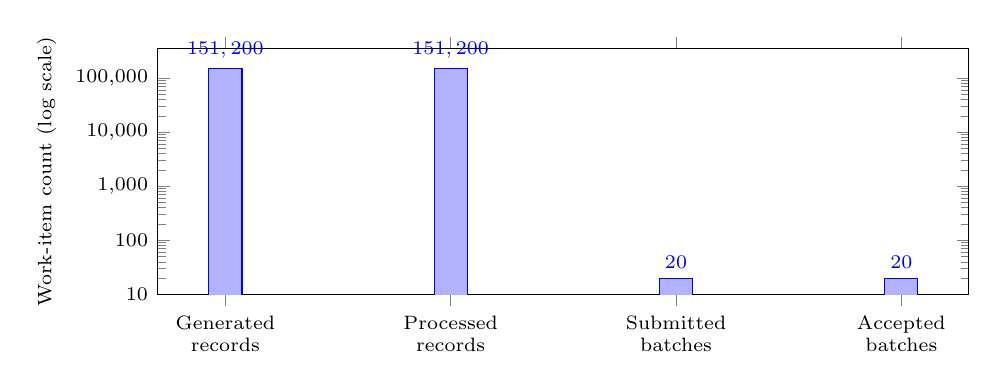
\begin{tikzpicture}
		\begin{axis}[
				ybar,
				ymode=log,
				log ticks with fixed point,
				width=0.98\columnwidth,
				height=4.7cm,
				ymin=10,
				ymax=350000,
				ytick={10,100,1000,10000,100000},
				xtick={1,2,3,4},
				xticklabels={{Generated\\records},{Processed\\records},{Submitted\\batches},{Accepted\\batches}},
				x tick label style={font=\scriptsize,align=center},
				y tick label style={font=\scriptsize},
				label style={font=\scriptsize},
				nodes near coords,
				point meta=rawy,
				nodes near coords style={font=\scriptsize,/pgf/number format/fixed,/pgf/number format/1000 sep={,}},
				bar width=12pt,
				ylabel={Work-item count (log scale)},
				fill=black!35,
				draw=black
			]
			\addplot coordinates {(1,151200) (2,151200) (3,20) (4,20)};
		\end{axis}
	\end{tikzpicture}
	\caption{Capacity-test outcomes. Generated/processed items are records; submitted/accepted items are batches.}
	\label{fig:capacity-results}
\end{figure}

Unauthorized requests with a missing or invalid token, or without an active \texttt{READ\_PGHD} capability, were rejected.
Inspection of PRE-bound payloads, IPFS objects, public IOTA metadata, denied responses, and relevant logs found no intelligible PGHD.
Changes to ciphertext, the recorded hash, signature, CID, IOTA metadata, or validity status were detected and rejected before the entry was treated as valid.
All required provenance fields were present for every tested source category.

\begin{table}[t]
	\caption{Non-Functional Evaluation}
	\label{tab:nf-results}
	\centering
	\scriptsize
	\begin{tabular}{@{}p{0.19\columnwidth}p{0.59\columnwidth}p{0.10\columnwidth}@{}}
		\toprule
		\shortstack[l]{\textbf{Test/}\\\textbf{property}} & \textbf{Observed evidence} & \textbf{Result} \\
		\midrule
		\textbf{NF01}\\Authorization & Missing, invalid, out-of-scope, expired, or revoked access returned neither PGHD nor key-opening material. & Pass \\
		\textbf{NF02}\\Confidentiality & No intelligible PGHD was found in inspected transit, IPFS, IOTA, denied responses, or logs. & Pass \\
		\textbf{NF03}\\Integrity & Changes to ciphertext, hash, signature, CID, metadata, and validity were detected and rejected. & Pass \\
		\textbf{NF04}\\Provenance & Patient, time, source, device/application, method, processing history, and validity were present. & Pass \\
		\textbf{NF05}\\Capacity & 151,200 records and 20 concurrent batches completed without loss or application failure. & Pass \\
		\textbf{NF06}\\Recovery & Unsent data persisted; after recovery, all tested units completed without observed duplication. & Pass \\
		\bottomrule
	\end{tabular}
\end{table}

During the recovery test, data remained locally available with a traceable failure state while connectivity or a supporting service was unavailable.
After service restoration, WorkManager retried the operation and every queued unit completed once in the tested run.
This result validates the implemented state and deduplication path for the injected failures, but it should not be generalized into a formal exactly-once guarantee across arbitrary distributed failures.

\FloatBarrier

\section{Discussion}

The results indicate that the architectural split is viable for DecMed.
Client-side encryption keeps PRE, IPFS, IOTA, and Redis outside the plaintext trust boundary.
The signed ciphertext hash lets both PRE and the clinician reject modifications, while the IPFS CID and IOTA state link stored content to an auditable metadata record.
PRE supports patient-controlled delegation without disclosing the patient's private key.
Finally, local persistence and batching decouple sensor collection from network and ledger availability.

Batching reduces remote operations but delays availability until a trigger fires.
Revocation blocks future key-material requests but cannot retract data already decrypted by a previously authorized clinician.
Provenance proves what the system recorded about origin and processing; it does not prove that a consumer wearable is clinically accurate.

The prototype was evaluated with one Android device, one wearable path, one PRE instance, a local IOTA/IPFS environment, and a desktop clinician client.
The 20-patient concurrency test was chosen to expose shared-object contention, not to model hospital-scale peak traffic.
The study does not report latency, energy consumption, ledger cost, long-duration reliability, or clinician usability.
Future work should evaluate asynchronous server queues, adaptive synchronization based on battery and network quality, larger multi-node deployments, credential recovery, interoperability with clinical data standards, and longitudinal use by patients and healthcare professionals.

\section{Conclusion}

This paper presented a PGHD module that extends DecMed from provider-generated records to patient-controlled, between-visit data.
The module combines offline-first local storage and batching with client-side AES-GCM encryption, SHA-256 and ECDSA integrity checks, PRE-based delegation, IPFS ciphertext storage, and IOTA-based access and validity metadata.
The prototype passed ten functional and six non-functional scenarios, processed 151,200 synthetic records without loss, and accepted 20 concurrent patient batches.
It also rejected the tested unauthorized and tampered requests and recovered queued data after temporary failures.
Within the stated prototype scope, the results support the feasibility of secure and traceable PGHD integration in DecMed.


\clearpage
\balance
\printbibliography

\end{document}
